\documentclass[12pt,twoside, a4paper, twocolumn]{article}
\usepackage[utf8]{inputenc}
\usepackage[brazil]{babel}
\usepackage[margin = 0.5in]{geometry}
\usepackage{amsmath}
\usepackage{amsthm}
\usepackage{amssymb}
\usepackage{amsthm}
\usepackage{setspace}
\usepackage[americanvoltages,fulldiodes,siunitx]{circuitikz}
\usepackage{lipsum}
\usepackage{pgfplots}
\usepackage{ifthen}
\usepackage{adjustbox}
\usepackage[section]{placeins}
\usepackage{hyperref}
\usepackage{graphicx}
\usepackage{amsmath}
\usepackage{amsthm}
\usepackage{amssymb}
\usepackage{amsthm}
\usepackage{setspace}
\usepackage[americanvoltages,fulldiodes,siunitx]{circuitikz}
\usepackage{lipsum}
\usepackage{pgfplots}
\usepackage{ifthen}
\usepackage{adjustbox}
\usepackage[section]{placeins}
\usepackage{hyperref}
\usepackage{graphicx}
\usepackage{adjustbox}
\pgfplotsset{compat=newest}
\graphicspath{ {./images/} }
%  #1 color - optional #2 x_0 #3 y_0 #4 x_f #5 y_f #6 name - optional  #7 true if adding lines to axis
\newcommand{\drawvector} [9] [color=cyan] {
\draw[line width=1.5pt,#1,-stealth](axis cs: #2, #3)--(axis cs: #4, #5) node[anchor=south west]{$#6$};
\ifthenelse{\equal{#7}{true}}{
\draw[line width=1pt,#1, dashed](axis cs: #4, #5)--(axis cs: #4, 0) node[anchor= north west]{$#8$};
\draw[line width=1pt,#1, dashed](axis cs: #4, #5)--(axis cs: 0, #5) node[anchor=south east]{$#9$};
}
{}
}
\newcommand\deriv[2]{\frac{\mathrm d #1}{\mathrm d #2}}
\title{Terceiro Relatório de Lab de Circuitos II}
\author{Henrique da Silva \\ hpsilva@proton.me}
\date{\today}
\pgfplotsset{width = 10cm, compat = 1.9}
\begin{document}
\maketitle
\pagenumbering{gobble}
\newpage
%pagenumbering{roman}
\tableofcontents
\newpage




\section{Introdução}








\subparagraph*{Neste relatório, vamos discutir calcular gráficos de Bode de dois circuitos de segunda ordem e medir suas características.}








\subparagraph*{Todos arquivos utilizados para criar este relatório, e o relatorio em si estão em:  \url{https://github.com/Shapis/ufpe_ee/tree/main/5th semester/Circuits II/}}
































\section{Análise preliminar}








\paragraph*{Utilizarei o WxMaxima e LTSpice para fazer a análise teórica do circuito antes de montá-lo fisicamente.}








\paragraph*{Após terminar as análises compararei os resultados obtidos nas análises numéricas e em laboratório para verificar sua coerência.}








\subsection{O Circuito}
\begin{adjustbox}{scale=0.30}
    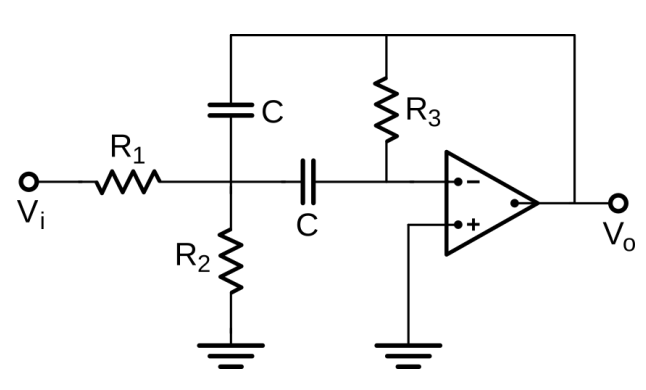
\includegraphics{AnaliseNodal.png}
\end{adjustbox}
\newpage
\subsection{WxMaxima}




\subsubsection{Análise geral do circuito}








\subparagraph*{Primeiro fiz manualmente a análise nodal do circuito que vamos construir, e passei ele para o domínio da frequência.}
\subparagraph*{}








\begin{adjustbox}{scale=0.4}
    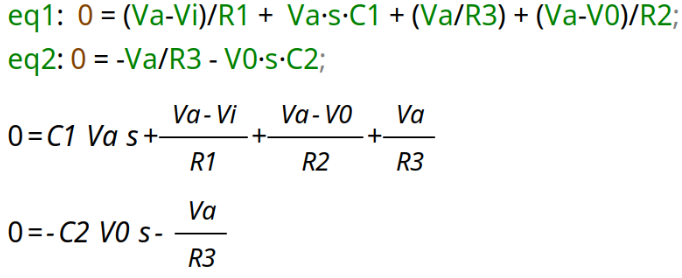
\includegraphics{eqs.png}
\end{adjustbox}








\subparagraph*{Após isso resolvi para $Va$ e $V_0$}








\subparagraph*{}








\begin{adjustbox}{scale=0.4}
    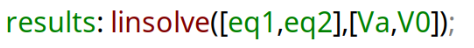
\includegraphics{linsolve.png}
\end{adjustbox}




\subparagraph*{}




\begin{adjustbox}{scale=0.4}
    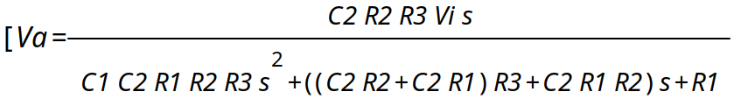
\includegraphics{va.png}
\end{adjustbox}




\subparagraph*{}




\begin{adjustbox}{scale=0.4}
    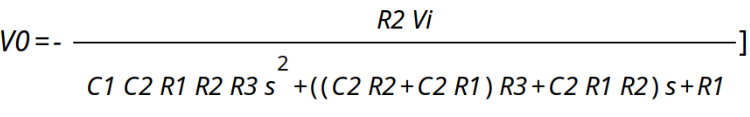
\includegraphics{v0.png}
\end{adjustbox}








\subparagraph*{Daqui criamos nossa função transferência $H$.}








\subparagraph*{}








\begin{adjustbox}{scale=0.4}
    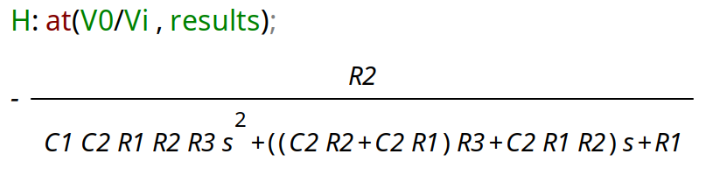
\includegraphics{H.png}
\end{adjustbox}








\subparagraph*{Agora com a função $H$ em mãos podemos substituir os valores dos resistores e do capacitor pelos que utilizaremos nos circuitos a serem analisados.}




\subsubsection{Análise do circuito 1}




\subparagraph*{Fazemos a substituição em $H$ dos valores que utilizaremos no circuito 1.}








\begin{equation*}
    \begin{aligned}
         & C_1  = 100nF          \\
         & C_2  = 10nF           \\
         & R_1  = 47k \varOmega  \\
         & R_2  = 470k \varOmega \\
         & R_3  = 470k \varOmega
    \end{aligned}
\end{equation*}








\subparagraph*{}








\begin{adjustbox}{scale=0.34}
    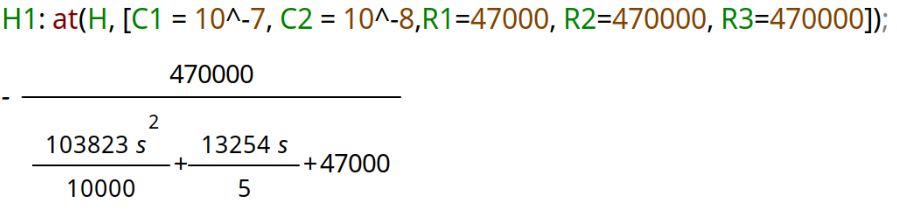
\includegraphics{H1.png}
\end{adjustbox}








\subparagraph*{Analisamos os pólos e zeros da função transferência e vemos que não há zeros. E os polos estão abaixo:}




\subparagraph*{}




\begin{adjustbox}{scale=0.5}
    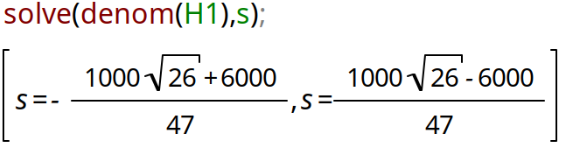
\includegraphics{H1denom.png}
\end{adjustbox}
















\subparagraph*{Agora faremos gráficos de Bode para analisar o comportamento da magnitude da função transferência e o ângulo de fase entre as saídas e entradas do circuito.}




\subparagraph*{}




\begin{figure}[h]
    \centering
    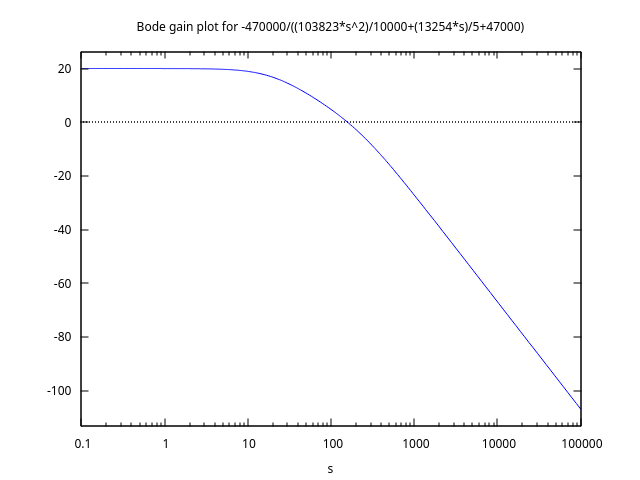
\includegraphics[width=1\columnwidth]{images/H1bodegain.png}
    \caption{Magnitude de H(s) do circuito 1.}
\end{figure}




\begin{figure}[h]
    \centering
    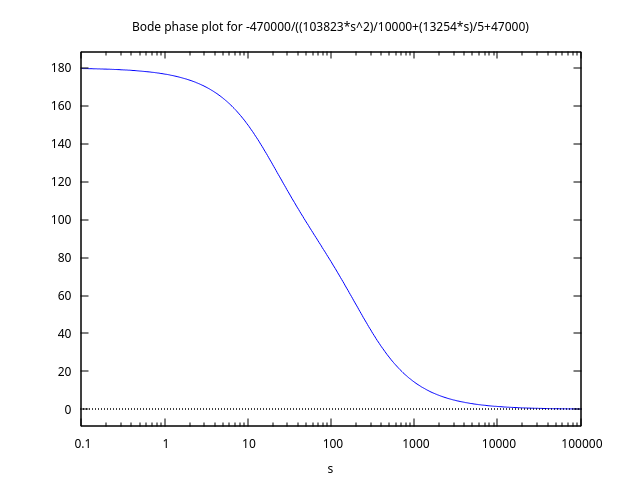
\includegraphics[width=1\columnwidth]{images/H1bodephase.png}
    \caption{Fase de H(s) do circuito 1.}
\end{figure}




\subparagraph*{}




\subparagraph*{Daqui retornei para o domínio do tempo para ter a função que descreve completamente o comportamento  da resposta do circuito.}
\pagebreak
\subparagraph*{}








\begin{adjustbox}{scale=0.35}
    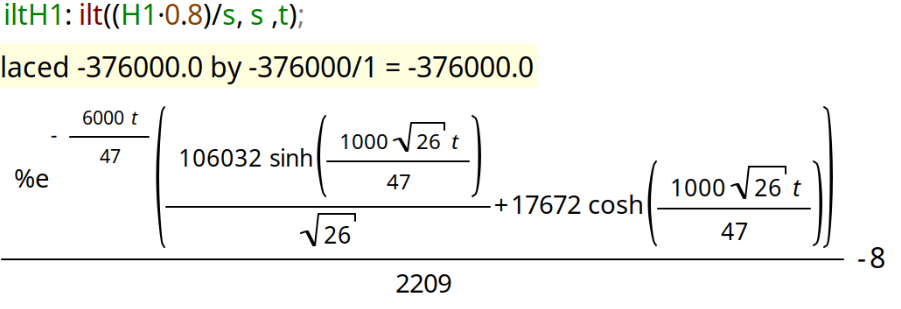
\includegraphics{iltH1.png}
\end{adjustbox}




\subparagraph*{Podemos ver que já que todos termos exceto o $-8$ dependem de uma exponencial negativa em $t$, então se nosso tempo tende a infinito, a resposta do circuito tende a $-8$.}




\subparagraph*{Fazendo esta análise numericamente abaixo verificamos este resultado.}




\subparagraph*{}




\begin{adjustbox}{scale=0.35}
    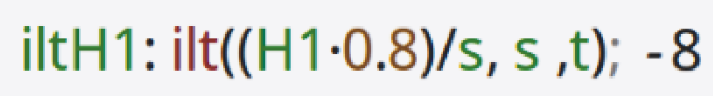
\includegraphics{limH1.png}
\end{adjustbox}




\subparagraph*{Com a função que descreve o comportamento do circuito no tempo em mãos, podemos montar seu gráfico e analisar seu comportamento a qualquer tempo.}
\subparagraph*{}




\begin{figure}[h]
    \centering
    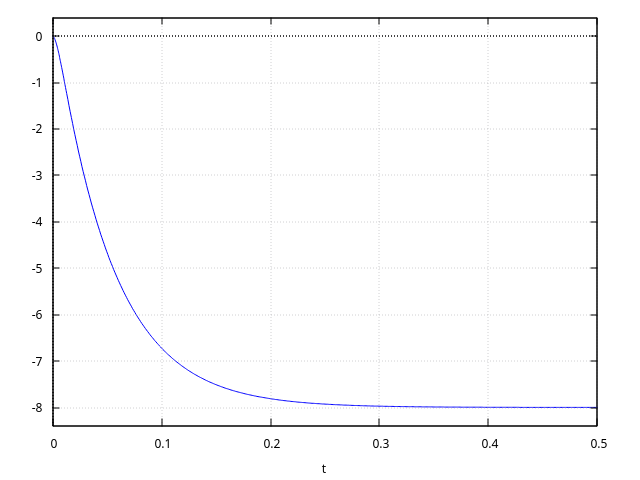
\includegraphics[width=1\columnwidth]{images/graficoH1t.png}
    \caption{Gráfico de $V_0$(t) do circuito 1.}
\end{figure}








\subparagraph*{Observamos que a função atinge valor final de $-8V$.}




\subparagraph*{E chega a $10\%$ deste valor em $9.2ms$ e $90\%$ em $122.2ms$.}




\subsubsection{Análise do circuito 2}




\subparagraph*{Fazemos a substituição em $H$ dos valores que utilizaremos no circuito 1.}








\begin{equation*}
    \begin{aligned}
         & C_1  = 100nF          \\
         & C_2  = 10nF           \\
         & R_1  = 470k \varOmega \\
         & R_2  = 470k \varOmega \\
         & R_3  = 47k \varOmega
    \end{aligned}
\end{equation*}








\subparagraph*{}








\begin{adjustbox}{scale=0.34}
    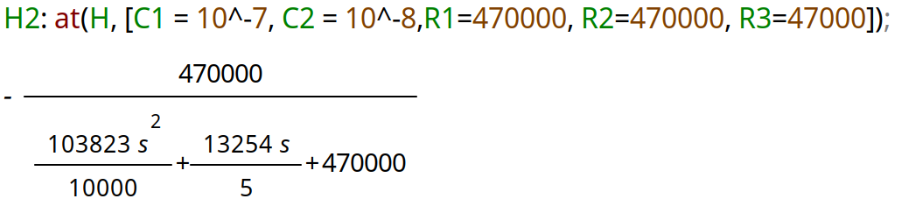
\includegraphics{H2.png}
\end{adjustbox}








\subparagraph*{Analisamos os pólos e zeros da função transferência e vemos que não há zeros. E os polos estão abaixo:}




\subparagraph*{}




\begin{adjustbox}{scale=0.5}
    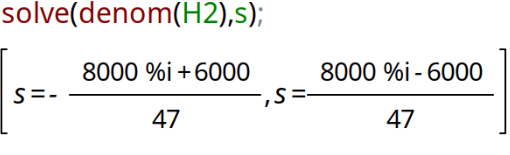
\includegraphics{H2denom.png}
\end{adjustbox}
















\subparagraph*{Agora faremos gráficos de Bode para analisar o comportamento da magnitude da função transferência e o ângulo de fase entre as saídas e entradas do circuito.}




\subparagraph*{}




\begin{figure}[h]
    \centering
    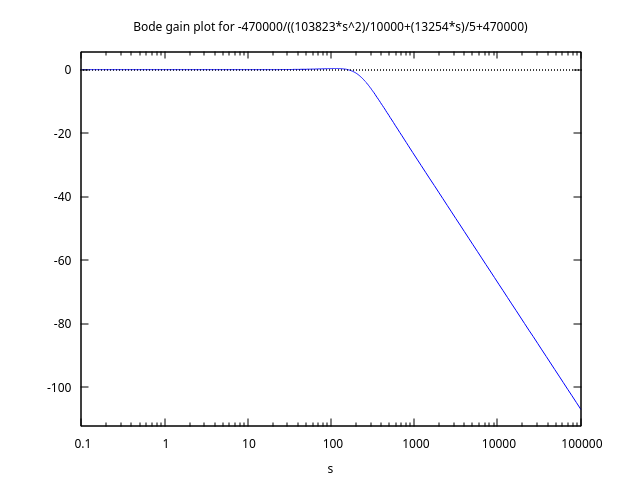
\includegraphics[width=1\columnwidth]{images/H2bodegain.png}
    \caption{Magnitude de H(s) do circuito 2.}
\end{figure}




\begin{figure}[h]
    \centering
    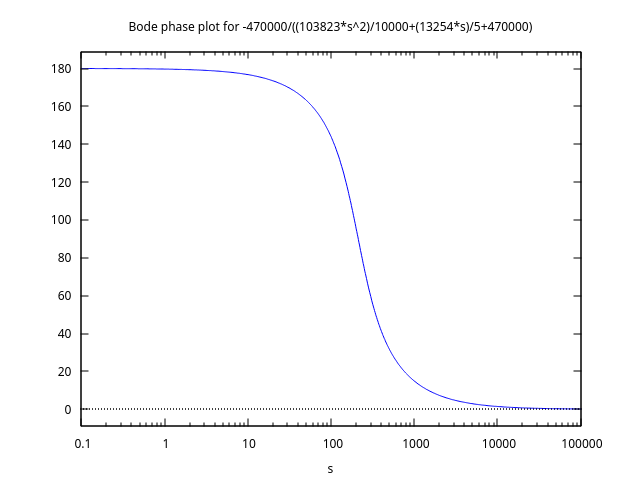
\includegraphics[width=1\columnwidth]{images/H2bodephase.png}
    \caption{Fase de H(s) do circuito 2.}
\end{figure}




\pagebreak




\subparagraph*{Daqui retornei para o domínio do tempo para ter a função que descreve completamente o comportamento  da resposta do circuito.}




\subparagraph*{}








\begin{adjustbox}{scale=0.35}
    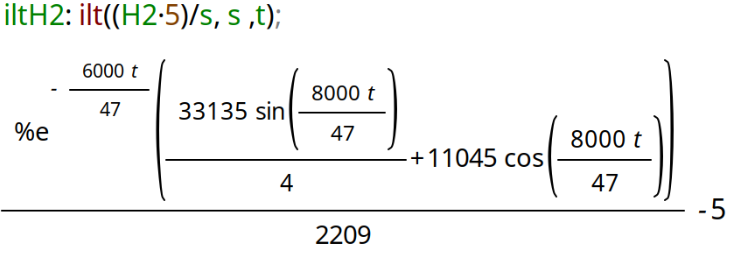
\includegraphics{iltH2.png}
\end{adjustbox}








\subparagraph*{Podemos ver que já que todos termos exceto o $-5$ dependem de uma exponencial negativa em $t$, então se nosso tempo tende a infinito, a resposta do circuito tende a $-5$.}




\subparagraph*{Fazendo esta análise numericamente abaixo verificamos este resultado.}




\subparagraph*{}




\begin{adjustbox}{scale=0.4}
    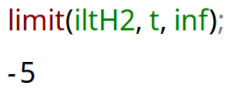
\includegraphics{limH2.png}
\end{adjustbox}




\subparagraph*{Com a função que descreve o comportamento do circuito no tempo em mãos, podemos montar seu gráfico e analisar seu comportamento a qualquer tempo.}




\newpage




\begin{figure}[h]
    \centering
    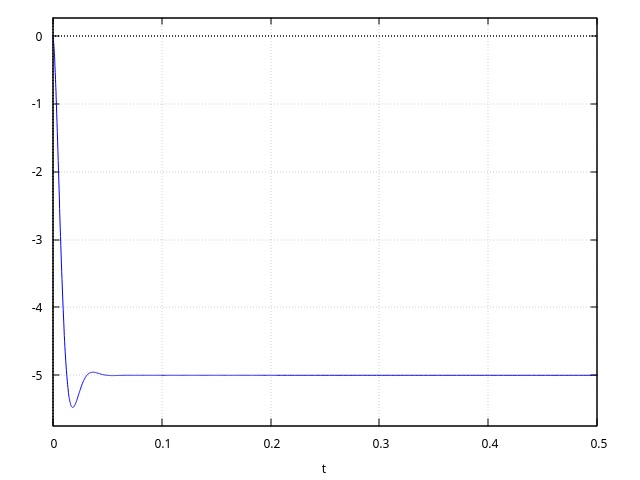
\includegraphics[width=1\columnwidth]{images/graficoH2t.png}
    \caption{Gráfico de $V_0$(t) do circuito 2.}
\end{figure}




\subparagraph*{Observamos que a função atinge valor final de $-5V$.}




\subparagraph*{E chega a $10\%$ deste valor em $2.4ms$ e $90\%$ em $10.9ms$.}




\subparagraph*{A partir de $10.9ms$ a função estará contida entre $90\%$ e $110\%$ do valor final.}












\newpage
















\subsection{LTSpice}




\subsubsection{Montagem do circuito}




\paragraph*{No LTSpice montaremos o circuito e geramos seus gráficos de Bode.}
\subparagraph*{}
\begin{adjustbox}{scale=0.11}
    \includegraphics{LTSPicecircuit.png}
\end{adjustbox}


\subsection{Circuito 1}


\begin{figure}[h]
    \centering
    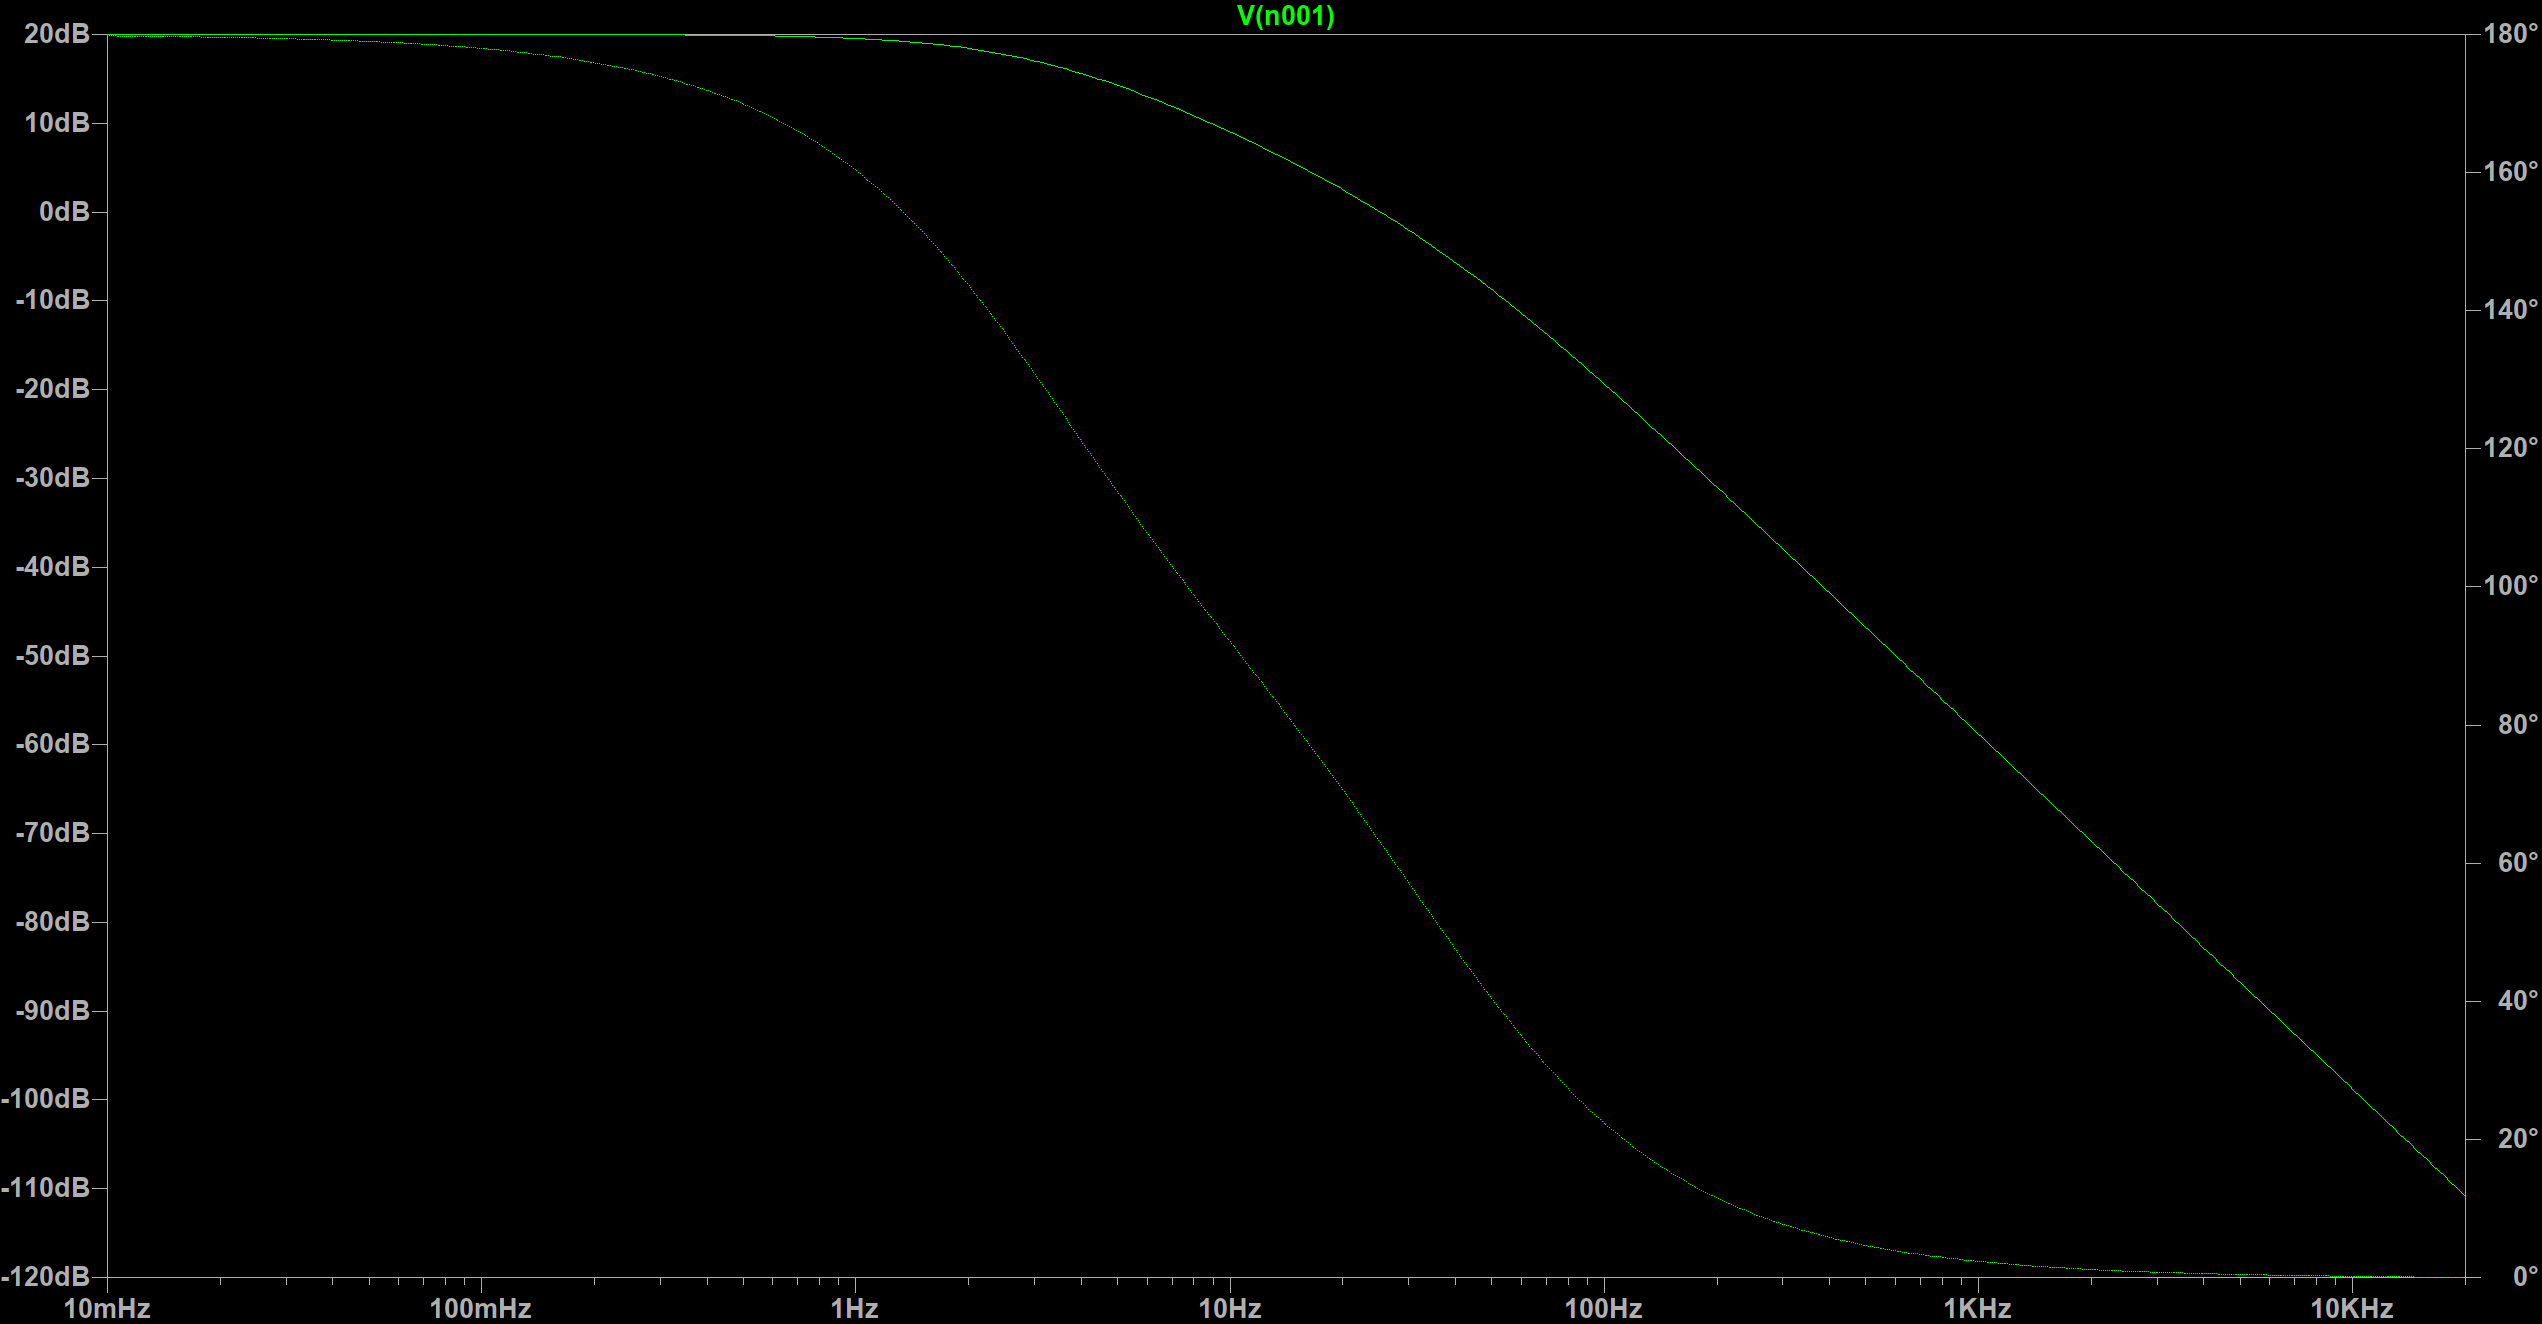
\includegraphics[width=1\columnwidth]{images/LTSpiceH1.png}
    \caption{Gráficos de Bode do circuito 1.}
\end{figure}


\subsection{Circuito 2}


\begin{figure}[h]
    \centering
    \includegraphics[width=1\columnwidth]{images/LTSPiceH2.png}
    \caption{Gráficos de Bode do circuito 2.}
\end{figure}


\newpage
\section{Medições em laboratório}








\paragraph{Vamos inicialmente fazer as medições dos componentes a serem usados.}








\subsection{Tabela de componentes}








\begin{equation*}
    \begin{aligned}
        C_1 & = 101.0nF           \\
        C_2 & = 10.5nF            \\
        R_1 & = 46.6 k \varOmega  \\
        R_2 & = 464.5 k \varOmega \\
        R_3 & = 474.2 k \varOmega \\
    \end{aligned}
\end{equation*}




\subsection{Circuito 1}


\subsubsection{Tabela de valores}


\subparagraph*{Encontrei $f_1 = 3$, daí segue os seguintes valores:}


\begin{center}
    \begin{tabular}{ |c|c|c|c| }
        \hline
        Múltiplos & Freq (Hz) & Entrada (V) & Saída (V) \\
        0.15      & $0.5$     & $1.67$      & $15.7$    \\
        0.4       & $1.2$     & $1.67$      & $14.6$    \\
        0.6       & $1.8$     & $1.67$      & $13.4$    \\
        0.8       & $2.4$     & $1.67$      & $12.1$    \\
        1.0       & $3.0$     & $1.67$      & $10.9$    \\
        1.2       & $3.6$     & $1.67$      & $9.9$     \\
        1.4       & $4.2$     & $1.67$      & $8.9$     \\
        1.8       & $5.4$     & $1.67$      & $7.4$     \\
        2.5       & $7.5$     & $1.67$      & $5.8$     \\
        4         & $12$      & $1.67$      & $3.6$     \\
        6         & $18$      & $1.67$      & $2.4$     \\
        10        & $30$      & $1.67$      & $1.3$     \\
        \hline
    \end{tabular}
\end{center}


\subsubsection{Função transferência}


\begin{figure}[h]
    \centering
    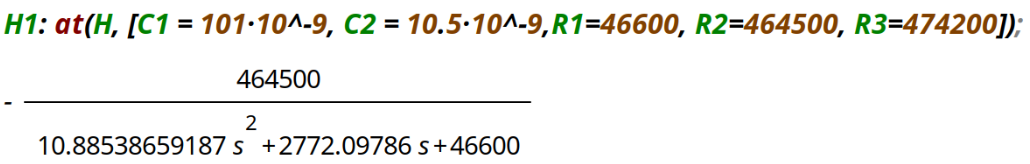
\includegraphics[width=1\columnwidth]{images/H1valoresreais.png}
    \caption{Função transferência do circuito 1.}
\end{figure}


\subsubsection{Estimativas experimentais de $ | H(jw) | $}


\begin{center}
    \begin{tabular}{ |c|c|c|c| }
        \hline
        Múltiplos & Freq (Hz) & $\mid H(jw) \mid$ \\
        0.15      & 0.5       & $9.4011$          \\
        0.4       & 1.2       & $8.7425$          \\
        0.6       & 1.8       & $8.0239$          \\
        0.8       & 2.4       & $7.2455$          \\
        1.0       & 3.0       & $6.5269$          \\
        1.2       & 3.6       & $5.9281$          \\
        1.4       & 4.2       & $5.3293$          \\
        1.8       & 5.4       & $4.4310$          \\
        2.5       & 7.5       & $3.4730$          \\
        4         & 12        & $2.1796$          \\
        6         & 18        & $1.4371$          \\
        10        & 30        & $0.7844$          \\
        \hline
    \end{tabular}
\end{center}


\subsubsection*{Escala log-log da magnitude de $H(jw)$ nos pontos experimentais}


\begin{figure}[h]
    \centering
    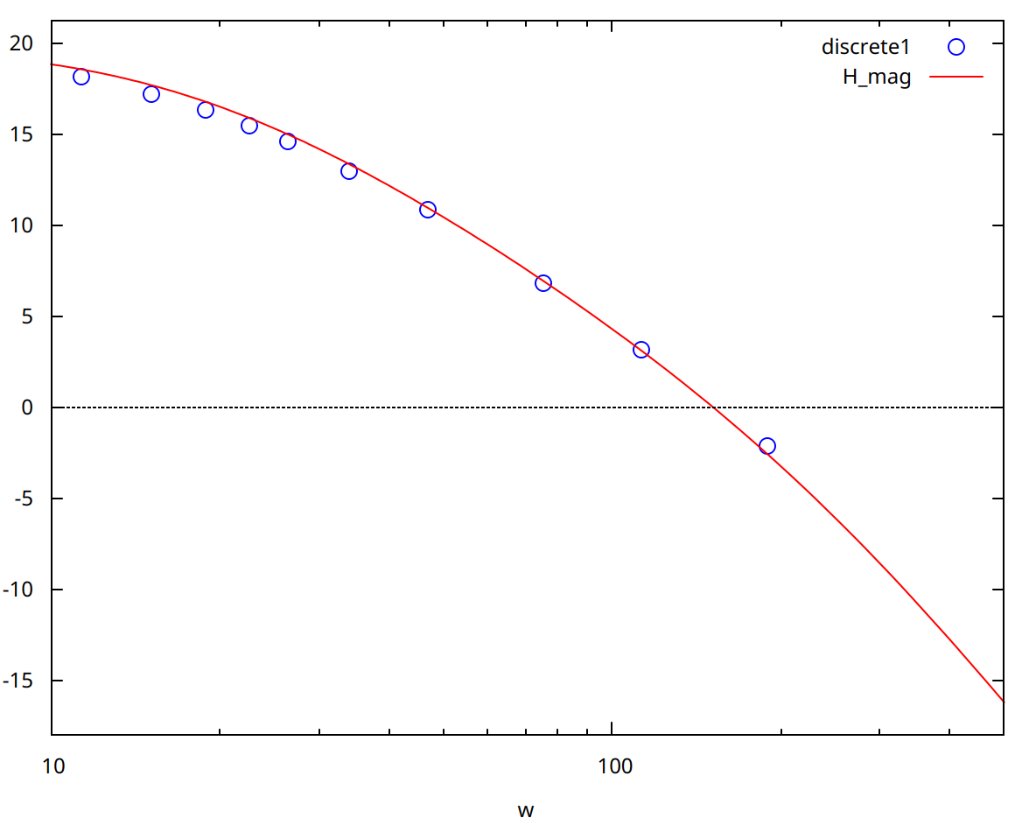
\includegraphics[width=1\columnwidth]{images/H1loglog.png}
    \caption{ $\mid H(jw) \mid$ por $w$ em escala log-log.}
\end{figure}




\subsubsection{Valores de corte}


\subparagraph*{Com entrada de $0.8V$ encontrei os seguintes valores de tempo para a onda atingir $10\%$  e $90\%$ do valor máximo respectivamente:}


\begin{equation}
    \begin{aligned}
        10\% & = 8.8ms   \\
        90\% & = 128.0ms
    \end{aligned}
\end{equation}




\newpage


\subsection{Circuito 2}


\subsubsection{Tabela de valores}


\subparagraph*{Encontrei $f_max = 15$, daí segue os seguintes valores:}


\begin{center}
    \begin{tabular}{ |c|c|c|c| }
        \hline
        Múltiplos & Freq (Hz) & Entrada (V) & Saída (V) \\
        0.15      & $2.2$     & $5.07$      & $4.9$     \\
        0.4       & $6$       & $5.07$      & $4.94$    \\
        0.6       & $9$       & $5.07$      & $4.94$    \\
        0.8       & $12$      & $5.07$      & $4.98$    \\
        1.0       & $15$      & $5.07$      & $5.03$    \\
        1.2       & $18$      & $5.07$      & $4.98$    \\
        1.4       & $21$      & $5.07$      & $4.94$    \\
        1.8       & $27$      & $5.07$      & $4.66$    \\
        2.5       & $37$      & $5.07$      & $3.66$    \\
        4         & $60$      & $5.07$      & $1.71$    \\
        6         & $90$      & $5.07$      & $0.76$    \\
        10        & $150$     & $5.07$      & $0.29$    \\
        \hline
    \end{tabular}
\end{center}


\subsubsection{Função transferência}


\begin{figure}[h]
    \centering
    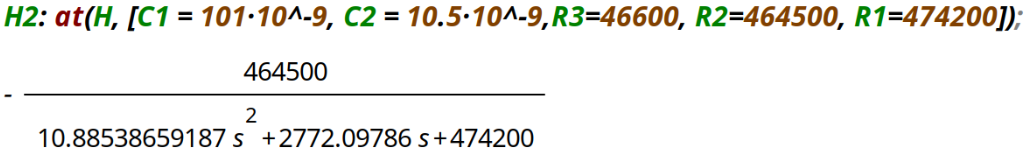
\includegraphics[width=1\columnwidth]{images/H2valoresreais.png}
    \caption{Função transferência do circuito 1.}
\end{figure}


\subsubsection{Estimativas experimentais de $ | H(jw) | $}


\begin{center}
    \begin{tabular}{ |c|c|c|c| }
        \hline
        Múltiplos & Freq (Hz) & $\mid H(jw) \mid$ \\
        0.15      & $2.2$     & $0.9667$          \\
        0.4       & $6$       & $0.9743$          \\
        0.6       & $9$       & $0.9743$          \\
        0.8       & $12$      & $0.9822$          \\
        1.0       & $15$      & $0.9921$          \\
        1.2       & $18$      & $0.9822$          \\
        1.4       & $21$      & $0.9743$          \\
        1.8       & $27$      & $0.9191$          \\
        2.5       & $37$      & $0.7218$          \\
        4         & $60$      & $0.3372$          \\
        6         & $90$      & $0.1499$          \\
        10        & $150$     & $0.0572$          \\
        \hline
    \end{tabular}
\end{center}
\pagebreak


\subsubsection*{Escala log-log da magnitude de $H(jw)$ nos pontos experimentais}


\begin{figure}[h]
    \centering
    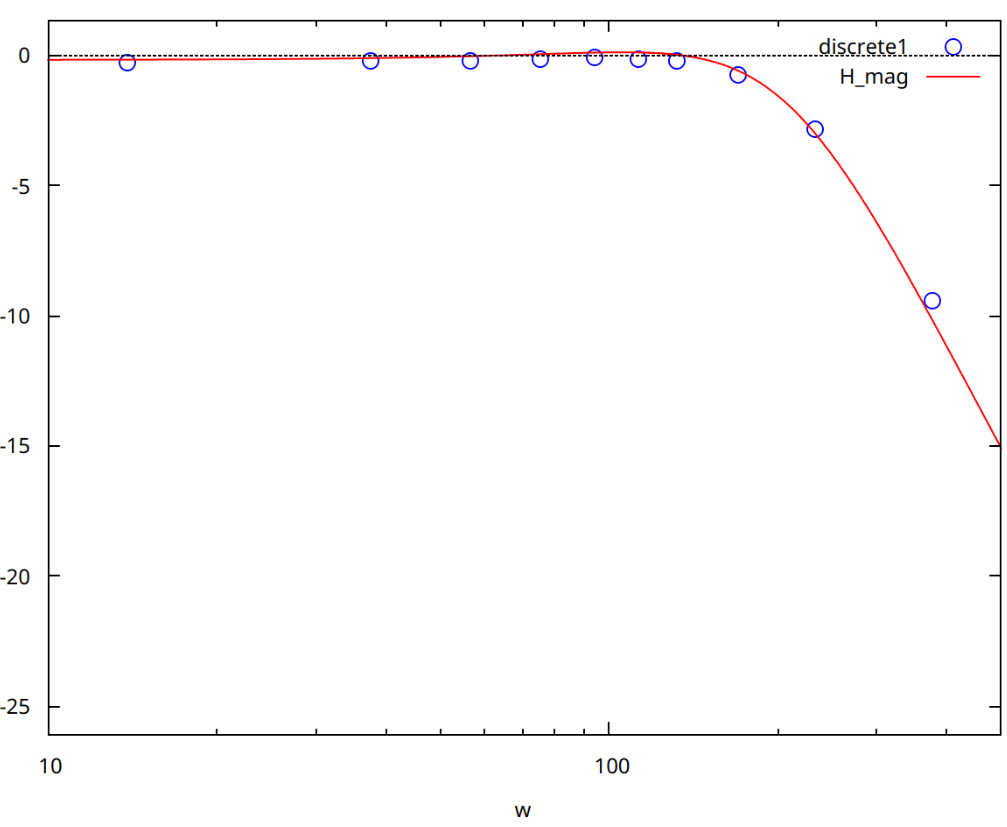
\includegraphics[width=1\columnwidth]{images/H2loglog.png}
    \caption{ $\mid H(jw) \mid$ por $w$ em escala log-log.}
\end{figure}




\subsubsection{Valores de corte}


\subparagraph*{Com entrada quadrada de $5V$ encontrei que apos $11ms$ a onda se enquadrada exclusivamente entre $90\%$ e $110\%$ do seu valor máximo.}


\newpage


\section{Conclusões}




\subparagraph*{Conseguimos com sucesso fazer a análise numérica por dois meios, utilizando o LTSpice e WxMaxima, e comparamos os resultados.}


\subparagraph*{Nos resultados práticos, a magnitude da função transferência foi coerente com os resultados esperados.}




\subparagraph*{Os gráficos que geramos a partir dos resultados experimentais foram coerentes com os gráficos gerados numericamente}


\subparagraph*{Mas em suma creio que tivemos sucesso em nos familiarizar com as ferramentas de análise de circuitos elétricos numéricos.}








\end{document}